\section{Installationsanleitung}

\subsection{DNA Center Installation}
Teile der nachfolgenden Installationsanleitung wurden aus den Anleitungen \cite{cisco-dna-installation-guide-1-2-chapter-configure}, \cite{cisco-dna-installation-guide}, \cite{cisco-dna-installation-guide-1-2-chapter-install} entnommen. Informationen die für die Installation nicht relevant sind, wurden weggelassen. 

Das DNA Center kann auf zwei verschiedene Modi aufgesetzt werden. Einerseits als Standalone Version oder als Cluster. Beim Cluster werden mehrere DNA Center Instanzen beziehungsweise Appliances benötigt. Diese Installationsanleitung behandelt nur die Variante \textit{Standalone}.

\subsection{CIMC Zugang aktivieren}
\paragraph{Schritt 1}
\label{installguide-cimc-step1}
~\\
Um die Installation über KVM durchzuführen zu können, muss zuerst Cisco IMC aktiviert werden. In unserem Fall macht das Cisco IMC DHCP. Die IP Adresse wird über die Leases auf dem DHCP Server ermittelt. (Siehe: \cite{cisco-dna-installation-guide-1-2-chapter-install}, \textit{Figure 2. DNA Center Rear Panel LEDs}). 

\paragraph{Schritt 2}
~\\
Anschliessend kann mit folgendem Link (\textit{\url{https://CIMC\_IP\_ADDRESS}}) auf die CIMC zugegriffen werden. Auf diesem muss mit den Standard Anmeldedaten (Benutzername: admin, Passwort: password) eingeloggt werden. 

\subsection{Konfiguration des Master Nodes}

\paragraph{Schritt 1}
~\\
Nachdem wie im vorherigen Abschnitt beschrieben im DNA Center eingeloggt wurde, kann im Cisco IMC \textit{Host Power $\rightarrow$ Power Cycle} gewählt und bestätigt werden.

\paragraph{Schritt 2}
~\\
Im Cisco IMC \textit{Launch KVM $\rightarrow$ Java based KVM} auswählen.

\paragraph{Schritt 3}
~\\
Nun wird der \textit{Maglev Configuration Wizard} angezeigt und es kann \textit{Start a DNA-C Cluster} ausgewählt werden.

\paragraph{Schritt 4}
~\\
Im nächsten Schritt muss die IP Konfiguration für die DNA Center Appliance angegeben werden. Es muss mindestens ein Interface konfiguriert und als Cluster Link definiert sein. Statische Routen können definiert werden, sind aber optional. Mit einem Klick auf Next erscheint der nächste Konfigurationsschritt im Wizard.

\begin{figure}[H]
	\centering
	\includegraphics[height=9cm]{img/sc_002.png}
	\caption{DNA Center Configuration Wizard - Entering Management IP}
	\label{fig:installguide-dna-center-install-step-4}
\end{figure} 

\paragraph{Schritt 5}
~\\
Anschliessend kann die virtuelle Cluster IP Adresse hinterlegt werden. Da es sich in diesem Fall um eine Standalone Installation handelt, kann dieser Schritt übersprungen werden.
\begin{figure}[H]
	\centering
	\includegraphics[height=9cm]{img/installguide/installguide-step11.PNG}
	\caption{Cisco - Maglev Configuration Wizard - Cluster Virtual IP Address}
	\label{fig:installguide-dna-center-install-step-11}
\end{figure} 

\paragraph{Schritt 6}
~\\
In diesem Schritt des Wizards werden alle User Account Einstellungen festgelegt. Hierbei ist zu beachten, dass das "Linux Password" für den SSH Zugriff benötigt wird und die "Administrator Passphrase" für den Zugang zum Web Interface. 

\begin{figure}[H]
	\centering
	\includegraphics[height=9cm]{img/sc_003.png}
	\caption{DNA Center Configuration Wizard - Entering Authentification Data}
	\label{fig:installguide-dna-center-install-step-13}
\end{figure}

\paragraph{Schritt 7}
~\\
In diesem Schritt wird der gewünschte NTP Server eingegeben. Im vorliegenden Fall \url{pool.ntp.org}.
\begin{figure}[H]
	\centering
	\includegraphics[height=9cm]{img/installguide/installguide-step14.PNG}
	\caption{Cisco - Maglev Configuration Wizard - NTP Server}
	\label{fig:installguide-dna-center-install-step-14}
\end{figure} 

\paragraph{Schritt 8}
~\\
Das DNA Center benötigt für das interne Netzwerk zwei Subnetze. Dazu müssen die entsprechenden Subnetze eingegeben werden, welche mindestens aus einem /21 bestehen. Diese Netzwerke müssen nicht von ausserhalb erreichbar sein.
\begin{figure}[H]
	\centering
	\includegraphics[height=9cm]{img/installguide/installguide-step16.PNG}
	\caption{Cisco - Maglev Configuration Wizard - Service Subnet}
	\label{fig:installguide-dna-center-install-step-16}
\end{figure} 

\paragraph{Schritt 9}
~\\
Der Wizard wird mit einem Klick auf \textit{next} oder \textit{proceed} abgeschlossen.

\paragraph{Schritt 10}
~\\
Nun wird das DNA Center aufgesetzt. \textbf{Achtung:} Dieser Prozess dauert mehrere Stunden. 

\begin{figure}[H]
	\centering
	\includegraphics[height=9cm]{img/sc_004.png}
	\caption{DNA Center Configuration Wizard - DNA Center uses docker}
	\label{fig:dna-center-install-step-install}
\end{figure}

\subsection{Einloggen im Web GUI}
Nachdem der \textit{Maglev Configuration Wizard} die Installation abgeschlossen hat, kann das DNA Center über das Webinterface aufgerufen werden.

Dazu wird mit einem gängigen Webbrowser die zuvor definierte IP-Adresse aufgerufen. In folgendem Fall \url{https://10.22.0.100}.

Anschliessend erfolgt das Login mit den im vorhergehenden Schritt definierten Anmeldedaten. 

\begin{figure}[H]
	\centering
	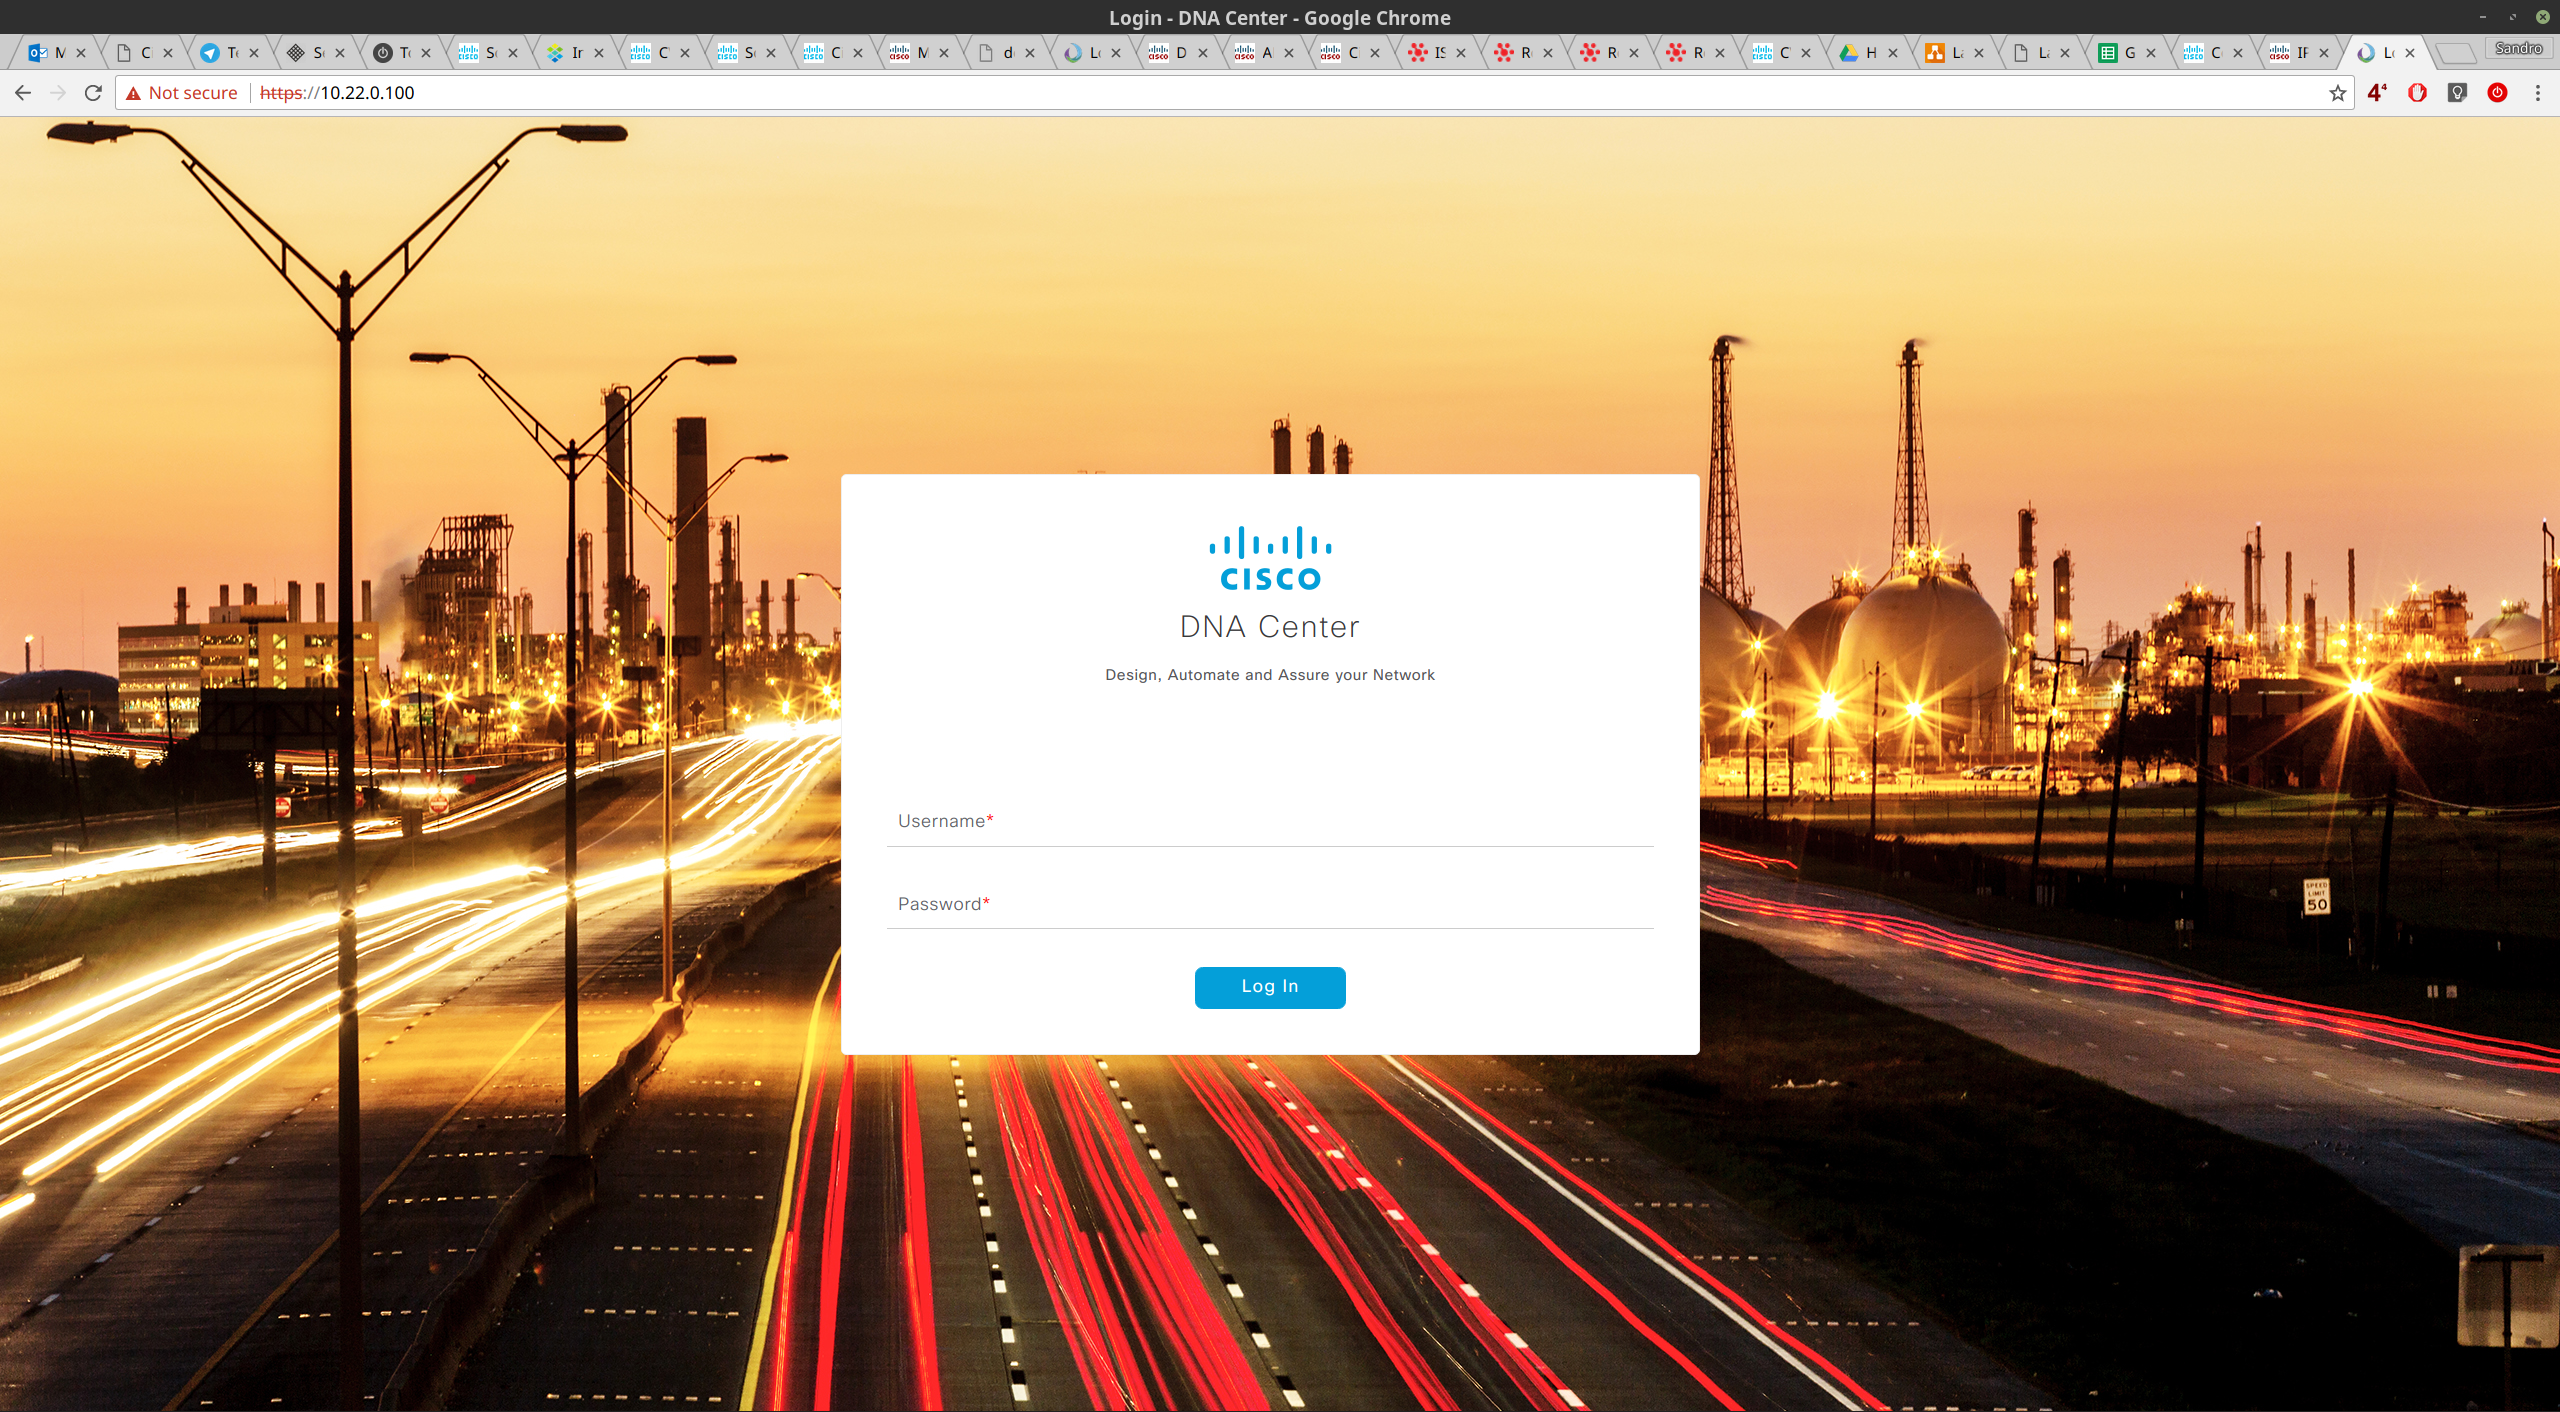
\includegraphics[height=9cm]{img/sc_005.png}
	\caption{DNA Center Web GUI - Login Seite im Webbrowser}
	\label{fig:installguide-dna-center-gui-1}
\end{figure}

\subsection{Cisco Credentials}
Gleich zu Beginn verlangt das DNA Center die Cisco Credentials, die mit dem Smart Account verknüpft sind, in welchem die Lizenzen verwaltet werden. Diese Informationen können auch zu einem späteren Zeitpunkt noch eingetragen werden.
\begin{figure}[H]
	\centering
	\includegraphics[height=9cm]{img/sc_006.png}
	\caption{DNA Center Web GUI - Cisco Credentials for Licences}
	\label{fig:installguide-dna-center-gui-2}
\end{figure}

\subsection{IP Address Manager - IPAM Server}

Im nächsten Schritt kann ein IPAM Server angegeben werden. Diese Einstellung ist optional und kann ebenfalls später angepasst werden. 

\begin{figure}[H]
	\centering
	\includegraphics[height=9cm]{img/sc_007.png}
	\caption{DNA Center Web GUI - Cisco IPAM - Enter Infoblox Credentials}
	\label{fig:installguide-dna-center-gui-3}
\end{figure}

\subsection{Terms and Conditions}
Im folgenden Abschnitt sind das \textit{Cisco End User Licence Agreement (EULA)} und alle weiteren relevanten \textit{Terms} aufmerksam zu lesen und mit \textit{Next} zu akzeptieren. 

\begin{figure}[H]
	\centering
	\includegraphics[height=7cm]{img/installguide/webgui-termsandcondition.png}
	\caption{DNA Center Web GUI - Terms and Conditions}
	\label{fig:installguide-dna-center-gui-4}
\end{figure}

\subsection{Abschluss}
Danach ist die initiale Konfiguration beendet und das DNA Center Dashboard wird angezeigt.

\begin{figure}[H]
	\centering
	\includegraphics[height=9cm]{img/sc_008.png}
	\caption{DNA Center Web GUI - Dashboard}
	\label{fig:installguide-dna-center-gui-5}
\end{figure}

\subsection{ISE Integration}
Für das Identity und Policy Management muss eine Cisco ISE integriert werden. Es gilt dabei zu beachten, dass die Cisco ISE in der richtigen Version vorliegen muss. Genauere Details dazu müssen der aktuellsten offiziellen Installationsanleitung von Cisco entnommen werden, da sich dies bei jedem Release ändern kann.
Damit eine Verknüpfung zwischen dem Cisco DNA Center und der Cisco ISE hergestellt werden kann, müssen im Cisco ISE zuerst einige Einstellungen vorgenommen werden. 
Die genauen Einstellungen für die ISE Integration können der folgenden Anleitung entnommen werden (Siehe: \cite{cisco-dna-appliance-installation-guide-release-1-chapter-post-installation-task}).

\subsubsection{ISE Vorbereiten}

\begin{enumerate}
	\item In Cisco ISE einloggen.
	\item \textit{Administration $\rightarrow$ Deployment} auswählen.
	\item Gewünschten ISE Node auswählen und in der nachfolgenden Ansicht \textit{Enable SXP Service}, \textit{Enable Passive Identity Service} und \textit{pxGrid} mit einem Haken anwählen
	\item Speichern drücken
	\item Im \textit{Profiling Configuration} Tab muss mindestens \textit{RADIUS} und \textit{SNMPQUERY} ausgewählt sein
	\item Unter \textit{Administration $\rightarrow$ Settings $\rightarrow$ ERS Settings} \textit{Enable ERS for Read/Write} auswählen und mit \textit{OK} bestätigen
\end{enumerate}

\subsubsection{Cisco ISE im DNA Center hinterlegen}
\begin{enumerate}
	\item In Cisco DNA Center Web GUI einloggen
	\item System Settings auswählen (Zahnrad oben rechts)
	\item Cisco ISE Panel auswählen
	\item \textit{Configure Setting} wählen
	\item Unter \textit{Settings- Auhentication and Policy Servers} auf das grosse Plus (+) drücken
	\item Im neuen Dialog Management IP Adresse, Shared Secret, Username, Password, FQDN und  Subscriber Name eingeben
	\item Update wählen
\end{enumerate}

\begin{figure}[H]
	\centering
	\includegraphics[height=9cm]{img/installguide/cisco-ise.png}
	\caption{Cisco ISE benötigte Konfigurationen für die DNA Center Verknüpfung}
	\label{fig:installguide-cisco-ise}
\end{figure}

